%-----------------------------------------------------------------------------------------------------------------
\section{Транспортная задача}
%-----------------------------------------------------------------------------------------------------------------
\subsection{Закрытая транспортная задача. Нахождение опорных планов}
Одной из задач линейного  программирования  является транспортная задача, состоящая, в общей постановке, в отыскании оптимального плана перевозок некоторого однородного груза с $m$ баз $A_1, A_2, \ldots , A_m$ $n$ потребителям $B_1, B_2, \ldots , B_n$. Пусть имеются определенные запасы груза на базах  $A_1, A_2, \ldots , A_m$, которые мы обозначим $a_1, a_2, \ldots , a_m$ соответственно. Заказы каждого из  потребителей (потребности) обозначим $b_1, b_2, \ldots , b_n$. Общее количество имеющегося груза обозначим $A (A = a_1 + a_2 + \ldots + a_m)$ , а общие потребности -- через $B (B = b_1 + b_2 + \ldots + b_n)$. При условии $A = B$ мы имеем закрытую модель, а при $A \neq B$ -- открытую модель транспортной задачи.

В этом параграфе мы рассмотрим закрытую транспортную задачу. Предположим, что базы и потребители соединены  коммуникациями, например железными дорогами. Обозначим стоимость перевозки единицы груза из пункта $A_i$ в пункт $B_j$ через $c_{ij}$. Числа $c_{ij}$ можно  расположить  в виде матрицы

\[ \left[\begin{array}{cccc}
a_{11}& a_{12} &\ldots & a_{1n}\\
a_{21}& a_{22} &\ldots & a_{2n}\\
\vdots& \vdots &\ddots & \vdots\\
a_{n1}& a_{n2} &\ldots & a_{nn}
\end{array}\right]\]

Эта матрица называется {\it матрицей стоимостей}. Задача заключается в нахождении такого плана перевозок, чтобы общая стоимость их была минимальной. При этом необходимо выполнить следующие два условия:

\begin{enumerate}
\renewcommand{\labelenumi}{\theenumi)}
\item все запасы груза должны быть вывезены;
\item заказы потребителей должны быть выполнены.
\end{enumerate}

Такие требования можно соблюсти лишь при условии $A = B$, то есть  в случае закрытой модели. Обозначим через $x_{ij}$ количество груза, которое планируется перевезти из пункта $A_i$ в пункт $B_j$. Эти величины  будут представлять собой переменные в нашей задаче. Их также можно расположить в виде матрицы, которая называется матрицей перевозок. Общая стоимость перевозок (целевая функция нашей задачи) имеет вид
\[z = \sum_{i,j}c_{ij}x_{ij}\]

Эту функцию требуется минимизировать. При этом, однако, величины $x_{ij}$ не  могут  принимать  произвольные  значения. Они {\it неотрицательны} и удовлетворяют следующим ограничениям, которые  выражают  требования 1) и 2), сформулированные выше:

$$\begin{cases}
x_{11} + x_{12} + \ldots + x_{1n} = a_1;\\
x_{21} + x_{22} + \ldots + x_{2n} = a_2;\\
\ldots \\
x_{m1} + x_{m2} + \ldots + x_{mn} = a_m.
\end{cases}
\begin{cases}
x_{11} + x_{12} + \ldots + x_{1n} = b_1;\\
x_{21} + x_{22} + \ldots + x_{2n} = b_2;\\
\ldots \\
x_{m1} + x_{m2} + \ldots + x_{mn} = b_m.
\end{cases}$$

Приведенная система ограничений состоит из двух подсистем, которые называются системой горизонтальных и вертикальных уравнений. Таким образом, закрытая транспортная задача является задачей линейного программирования с ограничениями равенствами. Система  ее  ограничений содержит $n + m$ уравнений с $n\cdot m$ неизвестными. Для решения транспортной задачи также применяют симплекс-метод, но в силу специфики задачи здесь можно обойтись без симплекс-таблиц. План перевозок с указанием запасов и потребностей, а также стоимостей перевозок, удобно записывать в виде таблицы данных:

\begin{figure}[h]
\center{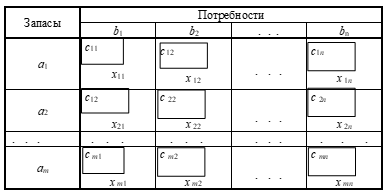
\includegraphics{pictures/picturefile_2_1}}
\end{figure}

Решение задачи можно получить путем некоторых преобразований этой таблицы, которые соответствуют переходу от одного  плана перевозок к другому. Как и в общем случае, оптимальное решение ищется среди опорных решений системы ограничений транспортной  задачи. Ранг этой системы равен $m + n - 1$, поэтому среди $m\cdot n$ переменных $x_{ij}$ выделяются $m + n - 1$ базисных переменных, а остальные $(m - 1)(n - 1)$ переменные являются свободными. В базисном решении свободные  переменные равны нулю. Обычно эти нули в таблицу не вписывают, оставляя соответствующие клетки пустыми. Таким образом, при внесении в  таблицу перевозок вместо $x_{ij}$  чисел, представляющих опорный план, мы имеем $m + n - 1$ заполненных   и $(m - 1)(n - 1)$ пустых клеток. Как и в общем случае, решение транспортной  задачи  начинается  с отыскания первого опорного плана (исходного опорного решения системы ограничений). Мы рассмотрим два метода построения такого опорного  плана. Суть обоих методов состоит в том, что опорный план составляется последовательно в несколько шагов (точнее, $m + n - 1$ шагов). На каждом из шагов заполняется одна клетка. При рассмотрении клетки с номерами $(k,r)$ на первом шаге может представиться три случая:

\begin{center}
а) $a_k > b_r$\\ б) $a_k = b_r$\\ в) $a_k < b_r$
\end{center}

В случае а) в клетку ставится число $b_r$, вычеркивается $r$-тый столбец, а запасы в пункте $A_k$ полагаются равными $a_k - b_r$. В случае в) в клетку  записывается число $a_k$, вычеркивается $k$-тая строка, а потребности в пункте $b_r$ полагаются равными $b_r - a_k$. В случае б) в клетку ставится число $a_k = b_r$ и вычеркивается, по выбору, строка или столбец (вычеркивать и строку, и столбец нельзя). Оставшиеся  потребности  в пункте $b_r$ или запасы в пункте $a_k$ полагаются равными нулю. После первого шага наша таблица сократилась на одну строку  или на один столбец, а потребности или запасы соответственно подправлены. В сокращенной таблице снова выбираем для заполнения  клетку и  повторяем все сначала. Начиная с первоначально  данной  таблицы и  повторив $m + n - 2$ раз описанный шаг, мы придем к “таблице”, состоящей из одной клетки. Заполнив эту последнюю клетку и совершив $m + n - 1$ шаг, мы получим искомый опорный план. Правда, мы не указали, каким образом на каждом шаге мы выбираем клетку для  заполнения. Различие  методов отыскания первого опорного плана как раз и состоит в различии способов выбора заполняемой клетки.

{\itМетод северо-западного угла}.  В этом методе на каждом шаге построения первого опорного плана заполняется верхняя левая клетка ("северо-западный угол") оставшейся таблицы.

{\itМетод наименьшей стоимости}. В этом методе на каждом шаге построения первого опорного плана заполняется та клетка оставшейся таблицы, которая имеет наименьший тариф $(c_{kr})$. Если такая клетка не единственная, то заполняется любая из них.

\primer{Найдем первый опорный план следующей транспортной  задачи методом северо-западного угла.}%Метка

\begin{figure}[h]
\center{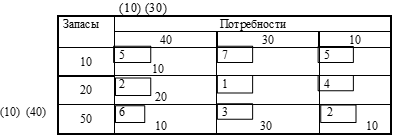
\includegraphics{pictures/picturefile_2_2}}
\end{figure}

В клетку $x_{11}$ ставим  10 и вычеркиваем строку. Потребности в $B_1$ станут равными 30. В клетку $x_{21}$ ставим 20 и вычеркиваем  строку. Потребности в $B_1$ равны 10. В клетку $x_{31}$ ставим 10 и  вычеркиваем столбец. В клетку $x_{32}$ ставим 30 и  вычеркиваем столбец. Запасы в $A_3$  станут равными 10. В клетку $x_{33}$ ставим 10. Процесс  нахождения  опорного плана окончен. Базисными переменными здесь будут $x_{11}, x_{21}, x_{31}, x_{32}, x_{33}$. Остальные переменные свободные.

Метод наименьшей стоимости дает здесь другой опорный план:

\begin{figure}[h]
\center{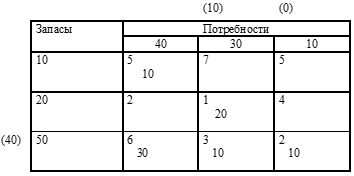
\includegraphics{pictures/picturefile_2_3}}
\end{figure}

Часто значение целевой функции на опорном плане, найденном методом наименьшей стоимости, меньше, чем на плане, полученном методом северо-западного угла. Этот опорный план как бы ближе к оптимальному. Хотя это и не всегда так, но часто нахождение оптимального решения, исходя из опорного плана, построенного методом наименьшей стоимости, требует меньше вычислений.
%-----------------------------------------------------------------------------------------------------------------
\subsection{Комбинаторные свойства циклов в матрице}
Под матрицей в этом параграфе понимается таблица, состоящая из клеток. {\itЦиклом} в матрице будем называть ломаную линию (рис. 2.1), звенья которой располагаются по строкам и столбцам матрицы, и которая удовлетворяет следующим двум условиям: %ссылка на рисунок

\begin{enumerate}
\renewcommand{\labelenumi}{\theenumi)}
\item эта ломаная является связной, т.е. из любой её вершины можно попасть в любую другую по звеньям ломаной;
\item в каждой вершине сходятся ровно два звена, причем одно из них располагается по строке, а другое по столбцу таблицы.
\end{enumerate}

Циклы в таблице могут иметь {\itсамопересечения}, т.е. звенья ломаной могут пересекаться в точке, не являющейся вершиной цикла (рис. 2.1, б). %ссылка на рисунок

\begin{figure}[h]
\center{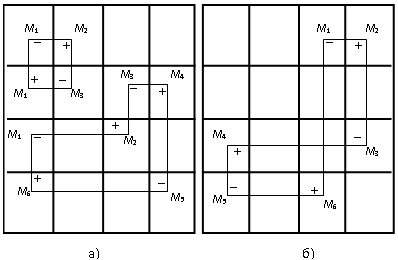
\includegraphics{pictures/picturefile_2_4}}
\caption*{Рис. 2.1. Примеры циклов в матрице}
\label{picture_2_1}
\end{figure}

Циклы в матрице обладают рядом свойств, которые описываются леммами 2.1 - 2.3. %ссылки на леммы

\lemma{Пусть дана матрица, состоящая из $n$ строк и $m$ столбцов, для которой выполнено неравенство $n\cdot m \ge n + m$. Если в этой матрице произвольно отмечено $n + m$ клеток, то существует цикл с вершинами в отмеченных клетках (быть может не во всех).}%метка

\so{Доказательство}. Докажем лемму по индукции, которую будем вести по величине $n + m$. Проверим утверждение леммы для случая $n + m = 4$. Для меньших значений не может выполняться неравенство $n\cdot m \ge n+m$. Единственной возможностью здесь является $n = m = 2$. Легко увидеть цикл, лежащий в четырех отмеченных клетках. Предположим, что утверждение доказано для всех матриц, для которых $n + m < p$ при некотором натуральномp. Докажем, что наше утверждение справедливо и при $n + m =  p$. Действительно, может представиться лишь две возможности

\begin{enumerate}
\renewcommand{\labelenumi}{\theenumi)}
\item для каждой отмеченной клетки в строке и в столбце матрицы находится другая отмеченная клетка;
\item есть хотя бы одна отмеченная клетка, в столбце или строке которой других отмеченных клеток нет.
\end{enumerate}

Рассмотрим вначале случай 2). Если есть отмеченная клетка, для которой нет других отмеченных клеток в строке (или столбце), то ее можно удалить, вычеркивая эту строку (или столбец). Получим матрицу, для которой $n + m < p$. По индуктивному предположению должен существовать цикл с вершинами в отмеченных клетках этой новой матрицы, и утверждение доказано. Если же имеет место случай 1), то из любой отмеченной клетки можно перейти в другую отмеченную клетку по строке (или столбцу). Из новой отмеченной клетки можно перейти в следующую и т. д. Поскольку клеток конечное число, то через ряд шагов мы вернемся в исходную клетку, то есть получим искомый цикл. Лемма 2.1 доказана. %ссылка

\lemma{Колчество вершин любого цикла в матрице четно.}%метка

\so{Доказательство}. Поскольку в каждой вершине сходится ровно два взаимно перпендикулярных звена, то при переходе через вершину звено поворачивается на угол $\pm \pi/2$. В результате обхода цикла суммарный угол поворота должен быть равен $2\pi q$, где $q\in Z$. Обозначим через $k$ количество вершин, в которых звено поворачивается на угол $\pi/2$, а через $l$ — количество вершин, в которых оно поворачивается на угол  $-\pi/2$. Тогда
$$\frac{\pi}{2}k - \frac{\pi}{2}l = 2\pi q     или     l = l = 4q$$
Поэтому количество всех вершин $k + l = (k - l) + 2l$ будет четным. Лемма 2.2 доказана.%ссылка

\opredelenie{Цикл в матрице называется означенным, если каждой вершине его сопоставлен знак «+» или «-», причем при обходе цикла знаки чередуются, т. е. если вершина имеет какой-то знак, то соседним вершинам сопоставляется противоположный знак (рис. 2.1, а), б)).}%метка и ссылка

Из леммы 2.2 следует, что любой цикл в матрице можно сделать означенным, причем двумя различными способами.%ссылка

\lemma{Во всяком означенном цикле число положительных вершин, лежащих в каждой строке или столбце, равняется количеству отрицательных вершин в этой строке или столбце.}%метка

\so{Доказательство}. Для каждой вершины в строке (столбце) имеется единственная соседняя вершина и для двух различных вершин в строке (столбце) соседние вершины различны. Рассмотрим положительные вершины в какой-нибудь строке (столбце). Для них в этой строке (столбце) имеется столько же соседних вершин. Они должны быть отрицательными по определению означенного цикла. Отсюда следует справедливость леммы 2.3.%ссылка
%-----------------------------------------------------------------------------------------------------------------
\subsection{Преобразование решения системы ограничений транспортной задачи сдвигом по означенному циклу}

Пусть имеется некоторое решение системы ограничений транспортной задачи. Запишем это решение в виде матрицы перевозок. Пусть в матрице перевозок задан некоторый означенный цикл.

\opredelenie{Сдвигом по означенному циклу на число $x$ матрицы перевозок называется такое преобразование этой матрицы, при котором меняются лишь элементы в клетках, где находятся вершины цикла, причем элемент в клетке с положительной вершиной увеличивается на число $x$, а элемент в клетке с отрицательной вершиной уменьшается на это же число.}%метка

\teorema{При сдвиге по означенному циклу на число x решение системы ограничений транспортной задачи переходит снова в решение этой же системы ограничений.}%метка

\so{Доказательство}. Рассмотрим горизонтальное уравнение, в котором слева стоит сумма элементов некоторой строки матрицы. Некоторые из этих элементов увеличиваются на число $x$, а некоторые уменьшаются на это же число. В силу леммы 2.3 количество положительных вершин в строке равно количеству отрицательных. Поэтому, если уравнение удовлетворялось до сдвига, то оно будет удовлетворяться и после сдвига, так как его левая часть не изменится. То же можно сказать и о каждом вертикальном уравнении. Теорема доказана.%ссылка на лемму

\lemma{Если матрица перевозок является базисным решением системы ограничений транспортной задачи, то не существует цикла с вершинами только в базисных клетках.} %метка

\so{Доказательство}. Переменные, отвечающие базисным клеткам, выражаются через переменные свободных клеток. Поэтому, если свободные переменные равны нулю, то базисные определяются однозначно. Предположим, что утверждение леммы неверно, т. е. существует цикл с вершинами в базисных клетках. Означим произвольно этот цикл и произведем сдвиг по нему на произвольное число $x$. Матрица останется решением системы ограничений транспортной задачи. При этом базисные переменные меняются, а свободные нет. Этого не может быть, так как базисные переменные определяются свободными однозначно. Лемма 2.4 доказана.%ссылка

\opredelenie{Циклом пересчета для данной свободной клетки называется означенный цикл, одна из вершин которого находится в данной свободной клетке, а  остальные — в  базисных  клетках. Цикл  пересчета означивается так, что вершине в данной свободной клетке приписывается знак «+».}%метка

\teorema{Для каждой свободной клетки опорного решения системы ограничений транспортной задачи существует цикл пересчета и притом только один.}%метка

\so{Доказательство}. Рассмотрим произвольную свободную клетку и добавим к ней $m + n - 1$ базисную клетку. Получим $m + n$ отмеченных клеток. Согласно лемме 2.1 существует цикл с вершинами в этих отмеченных клетках. Поскольку по лемме 2.4 нет цикла с вершинами в базисных клетках, то этот цикл должен иметь вершину в данной свободной клетке, т. е. существование цикла пересчета доказано. Если бы существовало два различных цикла пересчета для данной свободной клетки, то из них можно было бы скомбинировать цикл с вершинами только в базисных клетках, а это невозможно. Теорема доказана.%ссылки

Цикл пересчета является инструментом с помощью, которого производится переход от одного опорного решения к другому. Действительно, произведем сдвиг по циклу пересчета для некоторой свободной клетки на число $x$ равное наименьшей из перевозок, стоящих в клетках с вершинами, имеющими знак “-”. При этом, по крайней мере, одна из прежних базисных переменных имеет значение 0 и мы можем перевести ее в число свободных  переменных, сделав  вместо нее базисной ту переменную, которая была свободной. Решение, полученное в результате сдвига по циклу пересчета на выбранное число x, по-прежнему будет опорным, но отвечающим уже другому базисному виду системы ограничений.

\primer{Преобразуем первое опорное решение примера 2.1, вводя в качестве новой базисной переменной $x_{12}.$}%метка и ссылка на пример

Составляем цикл пересчета для клетки $x_{12}$. Минимальное  из  чисел, стоящих в клетках с отрицательными вершинами, равно 10. Производя сдвиг по циклу на число 10, получим новое опорное решение.

\begin{figure}[h]
\center{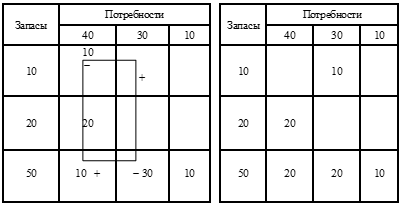
\includegraphics{pictures/picturefile_2_5}}
\end{figure}

%-----------------------------------------------------------------------------------------------------------------
\subsection{Нахождение коэффициентов при свободных переменных в базисном виде системы ограничений транспортной задачи}

Пусть система ограничений транспортной задачи приведена к базисному виду. Базисная переменная $x_{kl}$ выражается через свободные переменные, причем коэффициенты этого выражения определяет следующая

\teorema{Коэффициент при свободной переменной $x_{ij}$ в выражении для базисной переменной $x_{kl}$ может принимать лишь три возможных значения 0, 1 и -1. При этом
\begin{enumerate}
\renewcommand{\theenumi}{\asbuk{enumi}}
\renewcommand{\labelenumi}{\theenumi)}
\item этот коэффициент равен 0, если в клетке переменной $x_{kl}$ нет вершины цикла пересчета для переменной $x_{ij}$;
\item этот коэффициент равен 1, если в клетке переменной $x_{kl}$ положительная вершина цикла пересчета для переменной $x_{ij}$;
\item  этот коэффициент равен -1, если в клетке переменной $x_{kl}$ отрицательная вершина цикла пересчета для переменной $x_{ij}$;
\end{enumerate}} %метка


\so{Доказательство}. Пусть дан некоторый базисный вид и соответствующее базисное решение системы ограничений транспортной задачи. Рассмотрим базисную переменную $x_{kl}$  и свободную переменную $x_{ij}$. В базисном решении $x_{ij}$=0. Построим цикл пересчета для клетки $x_{ij}$ и произведем сдвиг рассматриваемого решения на некоторое число $x_0$. Получим новое решение системы ограничений транспортной задачи, в котором изменилась лишь одна свободная переменная $x_{ij}$. Поэтому базисная переменная получает новое значение  $x_{kl}^{(1)} = x_{kl} + qx_0$, где $q$ — является коэффициентом, с которым переменная $x_{ij}$ входит в выражение для $x_{kl}$. С другой стороны, это новое решение получено сдвигом по означенному циклу.  Поэтому  $q = 0$,  если в  клетке  $x_{kl}$  нет вершины цикла  пересчета  для  клетки $x_{ij}$; $q = 1$, если в клетке $x_{kl}$ — положительная вершина и $q = -1$, если в клетке $x_{kl}$ — отрицательная вершина. Теорема доказана.
%-----------------------------------------------------------------------------------------------------------------
\subsection{Выражение целевой функции транспортной задачи через свободные переменные}

В выражении целевой функции транспортной задачи ${z = \sum_{i,j}c_{ij}x_{ij}}$ суммирование распространяется на все клетки. Если система ограничений приведена к базисному виду, то базисные переменные можно из этого выражения исключить. Получим выражение
$$z = \gamma_0 + \sum_\text{св. пер.}\gamma_{ij}x_{ij},$$
где суммирование производится по свободным клеткам. Для дальнейшего важно знать коэффициенты $\gamma_{ij}$. Назовем {\it алгебраической суммой стоимостей по означенному циклу} в таблице данных транспортной задачи разность между суммой стоимостей в клетках с положительными вершинами и суммой стоимостей в клетках с отрицательными вершинами этого означенного цикла.

\teorema{Для любого базисного вида системы ограничений транспортной задачи коэффициент $\gamma_{ij}$ в выражении через свободные переменные целевой функции этой задачи равен алгебраической сумме стоимостей по циклу пересчета для свободной клетки $x_{ij}$.} %метка

\so{Доказательство}. Зафиксируем некоторую свободную переменную $x_{ij}$ и подсчитаем коэффициент $\gamma_{ij}$ для нее. В первоначальное выражение для $z$ переменная $x_{ij}$ входит непосредственно с коэффициентом $c_{ij}$, а также посредством базисных переменных. Если учесть теорему 2.3, то становиться очевидным, что каждая базисная переменная $x_{kl}$, в клетке которой есть вершина цикла пересчета для переменной $x_{ij}$, вносит в коэффициент $\gamma_{ij}$ слагаемое $\pm c_{kl}$. Причем, если в клетке $x_{kl}$ находится положительная вершина, то это слагаемое равно $c_{kl}$, а в случае отрицательной вершины — $(-c_{kl})$. Теорема 2.4 доказана. %ссылки
%-----------------------------------------------------------------------------------------------------------------
\subsection{Распределительный метод}

Этот метод, по сути, является симплекс-методом для транспортной задачи. При этом вычисления организуются без симплекс-таблиц, а используются циклы пересчета для всевозможных свободных клеток опорных решений. Пусть имеется первое опорное решение. В нем свободные переменные равны нулю. Мы переходим к другому опорному решению, увеличивая от нуля некоторую свободную переменную. Поскольку мы решаем задачу на минимум, то для уменьшения целевой функции нужно выбрать для увеличения от нуля ту свободную переменную, для которой $\gamma_{ij} < 0$. Увеличение выбранной переменной $x_{ij}$ нельзя производить неограниченно, поскольку решение может стать недопустимым. Граница увеличения $x_{ij}$ определяется способом перехода к следующему опорному решению. Этот переход мы производим с помощью цикла пересчета для клетки $x_{ij}$. Для того, чтобы сдвиг по циклу не привел к недопустимому решению, нужно следить за тем, чтобы базисные переменные не стали отрицательными. Для этого просматривают клетки цикла пересчета с отрицательными вершинами и выбирают среди них ту, в которой стоит минимальная величина перевозки. Эта клетка и определяет базисную переменную, которую мы выведем из числа базисных, вводя вместо нее переменную $x_{ij}$. Порядок работы по распределительному методу можно описать следующим образом:

\begin{enumerate}
\item Находится первое опорное решение одним из рассмотренных выше способов.
\item Для каждой свободной клетки строим цикл пересчета и определяем коэффициент $\gamma_{ij}$ как алгебраическую сумму стоимостей по циклу пересчета. Если все коэффициенты $\gamma_{ij} \ge 0$, то задача решена и найденное опорное решение является точкой минимума задачи. В противном случае переходим к пункту 3.
\item Выбираем свободную клетку с отрицательным значением $\gamma_{ij}$ и рассматриваем величины перевозок в клетках с отрицательными вершинами цикла пересчета для $x_{ij}$. Из этих перевозок выбираем наименьшую, которую обозначим через $x$.
\item Производим сдвиг по циклу пересчета для клетки, выбранной в пункте 3 на число $x$. Получаем новое опорное решение, на котором значение целевой функции будет меньше, чем на старом.
\item Переходим к пункту 2, то есть снова подсчитываем коэффициенты $\gamma_{ij}$ для новых свободных клеток. Описанные шаги производятся до тех пор, пока на очередном шаге все коэффициенты $\gamma_{ij}$ не станут неотрицательными.
\end{enumerate}
%-----------------------------------------------------------------------------------------------------------------
\subsection{Метод потенциалов}

В распределительном методе наиболее трудоемкой частью является подсчет коэффициентов $\gamma_{ij}$ для каждой свободной клетки. Существует метод, позволяющий подсчитывать эти коэффициенты без составления циклов пересчета. Этот метод называется методом потенциалов.

Каждому  пункту отправления (базе) $A_i$ сопоставим величину $u_i$ (потенциал пункта отправления), каждому потребителю $B_j$ сопоставим потенциал $v_j$. Будем находить эти потенциалы из того условия, что {\it для каждой базисной клетки $x_{kl}$ сумма потенциалов равна стоимости в этой клетке}
$$u_k + v_l = c_{kl}.$$

Поскольку базисных клеток $m + n - 1$, то мы имеем систему $m + n - 1$  уравнений с $m + n$ неизвестными. Эта система имеет бесконечно много решений. Если положить один из потенциалов равным нулю, то мы легко найдем некоторое решение этой системы уравнений.

\teorema{Для любой свободной клетки $x_{ij}$ алгебраическая сумма стоимостей по циклу пересчета $\gamma_{ij}$ равна разности между стоимостью в этой клетке и  суммой соответствующих потенциалов
$$\gamma_{ij} = c_{ij} - (u_i + v_j)$$} %метка

\so{Доказательство}. Будем обходить цикл пересчета, выйдя из свободной клетки $x_{ij}$, например, по столбцу. Сначала мы попадем в базисную клетку $x_{kj}$, расположенную в $k$-ой строке и в том же $j$-ом столбце, что и клетка $x_{ij}$. Затем, двигаясь по $k$-ой строке, мы перейдем из клетки $x_{kj}$ в базисную клетку $x_{kl}$, расположенную в $l$-ом столбце и в той же $k$-ой строке, что и клетка $x_{kj}$, и т. д. Наконец, выйдя из некоторой базисной клетки $x_{iv}$, лежащей в $v$-ом столбце, мы вернемся, и при том по $i$-ой строке, в свободную клетку $x_{ij}$, так как вышли из нее по столбцу. Получаем следующую последовательность клеток (стрелки указывают направление обхода)
$$x_{ij} \to x_{kj} \to x_{kl} \to x_{sl} \to \ldots \to x_{uv} \to x_{iv}.$$

Составим алгебраическую сумму стоимостей $\gamma_{ij}$ по этому циклу пересчета.
$$\gamma_{ij} = c_{ij} - c_{kj} - c_{kl} - c_{sl} + \ldots + c_{uv} - c_{iv}.$$

Все клетки, кроме $x_{ij}$, в этом цикле являются базисными. Поэтому все стоимости, кроме $c_{ij}$, равны суммам соответствующих потенциалов и $\gamma_{ij} = c_{ij} - (u_k + v_j) + (u_k + v_l) - (u_s + v_l) + \ldots + (u_u + v_v) - (u_i + v_v)$.

После раскрытия скобок все потенциалы, кроме $u_i$ и $v_j$ уничтожаются и $\gamma_{ij} = c_{ij} - (u_i + v_j)$, что и требовалось доказать.

{\it Опираясь на порядок работы по распределительному методу, сформулируем правила работы по методу потенциалов.}

\begin{enumerate}
\item Нахождение первого опорного решения.
\item Нахождение потенциалов пунктов отправления и назначения.
\item Нахождение коэффициентов $\gamma_{ij} = c_{ij} - (u_i + v_j)$ для свободных клеток. Если все $\gamma_{ij} \ge 0$, то данное опорное решение является оптимальным и задача решена. В противном случае переходим к пункту 4).
\item  Выбор свободной клетки с $\gamma_{ij} < 0$. Построение цикла пересчета для выбранной клетки. Сдвиг по этому циклу опорного решения на величину минимальной перевозки среди тех, что стоят в клетках с отрицательными вершинами цикла пересчета. Получение нового опорного решения. Переход к пункту 2.
\item Операции, указанные в пунктах 1) — 4) повторяются до тех пор, пока величины $\gamma_{ij}$ для всех свободных клеток не станут неотрицательными. Соответствующее опорное решение будет точкой минимума транспортной задачи.
\end{enumerate}

\primer{Решить следующую транспортную задачу, находя первое опорное решение методом наименьшей стоимости.} %метка

\begin{figure}[h]
\center{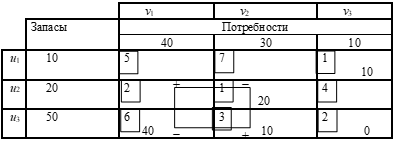
\includegraphics{pictures/picturefile_2_6}}
\end{figure}

Составляем и решаем систему уравнений для потенциалов по базисным клеткам:

$$\begin{cases}
u_1 + v_3 = 1,\\u_2 + v_2 = 1,\\u_3 + v_1 = 6,\\u_3 + v_2 = 3,\\u_3 + v_3 = 2;
\end{cases}
\begin{cases}
u_1 = -1,\\u_2 = -2,\\ u_3 = 0;
\end{cases}
\begin{cases}
v_1 = 6,\\v_2 = 3,\\v_3 = 2;
\end{cases}$$

Здесь мы положили $u_3 = 0$ и решили систему. Для каждой свободной клетки вычисляем $\gamma_{ij}$.

\begin{gather*}
\gamma_{11} = 5 - (-1 + 6) = 0;\\\gamma_{12} = 7 - (-1 + 3) = 5;\\\gamma_{21} = 2 - (-2 + 6) = -2;\\\gamma_{23} = 4 - (-2 + 2) = 4.
\end{gather*}

Имеется одна свободная клетка $x_{21}$ с отрицательным $\gamma_{21} = -2$. Строим цикл пересчета для этой клетки. Наименьшее число, стоящее в клетках с отрицательными вершинами, равно 20. Производим сдвиг на 20 по этому циклу пересчета. Получаем новое опорное решение.

\begin{figure}[h]
\center{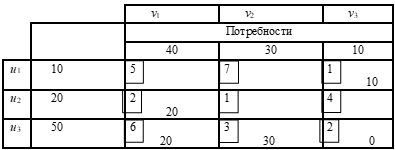
\includegraphics{pictures/picturefile_2_7}}
\end{figure}

Снова составляем систему уравнений для потенциалов:
$$\begin{cases}
u_1 + v_3 = 1,\\u_2 + v_1 = 2,\\u_3 + v_1 = 6,\\u_3 + v_2 = 3,\\u_3 + v_3 = 2;
\end{cases}
\begin{cases}
u_1 = -1,\\u_2 = -4,\\ u_3 = 0;
\end{cases}
\begin{cases}
v_1 = 6,\\v_2 = 3,\\v_3 = 2;
\end{cases}$$

Снова подсчитываем коэффициенты $\gamma_{ij}$ для свободных клеток:

\begin{gather*}
\gamma_{11} = 5 - (-1 + 6) = 0;\\\gamma_{12} = 7 - (-1 + 3) = 5;\\\gamma_{21} = 1 - (-4 + 3) = 2;\\\gamma_{23} = 4 - (-4 +2) = 6.
\end{gather*}

Здесь все коэффициенты неотрицательны. Это означает, что последнее опорное решение является оптимальным. При этом $z_{min} = 1\cdot10 + 2\cdot20 + 6\cdot20 + 3\cdot30 + 2\cdot0 = 260$.   Координаты   точки  минимума: $х_{11} = 0; х_{12} = 0; х_{13} = 10; х_{21} = 20;  х_{22} = 0; х_{23 }= 0; х_{31} = 20; х_{32} = 30; х_{33} = 0$.





%разделитель
\subsection{Об одном свойстве закрытой транспортной задачи}
Матрицу стоимостей транспортной задачи можно определенным образом изменить, не меняя оптимального плана перевозок. Справедлива следующая \teorema{Если к элементам произвольного столбца или
произвольной строки матрицы стоимостей транспортной задачи
прибавить одно и то же произвольное число, то целевая функция
задачи изменится на постоянное слагаемое. Таким образом,
получаются две транспортные задачи с разными матрицами
стоимостей, но одинаковыми оптимальными планами.}

\so{Доказательство}. Пусть дана транспортная задача с матрицей стоимостей $C=(c_{ij})$ . Рассмотрим транспортную задачу c другой матрицей стоимостей $C_1=(c_{ij}+\alpha_i+\beta_j)$, где $\alpha_i(i=1,\,...,n)$ и$\beta_j(j=1,\,...,m)$ - произвольные числа. Запишем целевую функцию второй задачи
\begin{center}
$z{}_{1}$=$\sum _{i,j}(c_{ij} +\alpha _{i} +\beta _{j} )x_{ij} = \sum _{i,j}c_{ij} x_{ij} +\sum _{i=1}^{n}\alpha _{i}  \sum _{j=1}^{m}x_{ij}  +\sum _{j=1}^{m}\beta _{j}  \sum _{i=1}^{n}x_{ij}   $.
\end{center}
Учитывая горизонтальные и вертикальные уравнения системы ограничений, получим
\begin{center}
$z{}_{1}$=$\sum _{i,j}c_{ij} x_{ij} +\sum _{i=1}^{n}\alpha _{i}  a_{i} +\sum _{j=1}^{m}\beta _{j}  b_{j} =z+ \sum _{i=1}^{n}\alpha _{i}  a_{i} +\sum _{j=1}^{m}\beta _{j}  b_{j} $,
\end{center}

что и доказывает утверждение теоремы. Очевидно, что оптимальные планы перевозок задач с матрицами перевозок $C$ и $C{}_{1}$ совпадают.

Сформулированное свойство транспортной задачи позволяет использовать преобразование матрицы перевозок для нахождения оптимального опорного решения. Можно так изменить элементы матрицы стоимостей, чтобы они, оставаясь неотрицательными, стали равными нулю в базисных клетках некоторого опорного плана. На этом основан так называемый венгерский метод решения транспортной задачи (см. \cite{literature_golshtein_1}, с.180).

\subsection{Открытые транспортные задачи}
Выше мы предполагали, что общие запасы $A$ равны общим потребностям $B$. В случае $A\neq B$  формулировка транспортной задачи различна  в  случаях $A<B$ и $A>B$. В случае$A<B$ мы можем обеспечить вывоз груза из пунктов отправления, однако удовлетворить все пункты назначения (потребителей) мы не можем. При  математической формулировке горизонтальные уравнения остаются без изменений, а вертикальные уравнения  превратятся в неравенства типа ''$\leq$``. Транспортная задача будет формулироваться так:
%для того, чтобы часть формул не была на другой странице
\nopagebreak{
\[z=\sum _{(i,j)}c_{ij} x_{ij} \to \min ; \]

\begin{equation*}
\begin{cases}
{l} {x_{11} +x_{12} +...+x_{1\, n} =a_{1} ,} \\
 {\cdots \cdots \cdots \cdots \cdots \cdots \cdots \cdots \cdots  } \\
{x_{m\, 1} +x_{m\, 2} +...+x_{m\, n} =a_{m} ;}
\end{cases}
\end{equation*}

\begin{equation*}
\begin{cases}
{l} {x_{11} +x_{21} +...+x_{m\, 1} \le b_{1} ,} \\
 {\cdots \cdots \cdots \cdots \cdots \cdots \cdots \cdots \cdots \cdots } \\
 {x_{1n} +x_{2\, n} +...+x_{m\, n} \le b_{n} ;}
\end{cases}
\end{equation*}
\begin{center}
$x_{ij} \ge 0,\quad i=\overline{1,m};\quad j=\overline{1,n}$
\end{center}}

В случае $A>B$ горизонтальные уравнения превращаются в неравенства, то есть система ограничений  состоит из первой группы неравенств и второй группы равенств. Если в условиях открытой транспортной задачи все пункты отправления и назначения равноправны, то такая задача легко сводится к закрытой транспортной задаче. Равноправие пунктов понимается в том смысле, что нет потребителей, которых  необходимо  обязательно удовлетворить (при $A<B$), и нет баз, которые необходимо  обязательно  освободить  от груза (при $A>B$).

Для сведения нашей  задачи к закрытой транспортной задаче в случае $A<B$ введем фиктивный пункт отправления  $A_{m+1}$ с запасами
\[a_{m+1} =\sum _{j=1}^{n}b_{j}  -\sum _{i=1}^{m}a_{i}  .\]

Рассмотрим закрытую задачу с пунктами отправления $A_{1}$, $A_{2}$, ... $A_{m}$, $A_{m+1}$  и с теми же пунктами назначения $B_{1}$, $B_{2}$, ..., $B_{n}$. В клетках, отвечающих  фиктивному пункту $A_{m+1}$, стоимости будем считать равными 0. Решение этой закрытой задачи даст решение нашей исходной задачи. Перевозки, отвечающие фиктивному пункту, имеют смысл недопоставок груза  соответствующим потребителям. В случае $A>B$ следует ввести фиктивный пункт назначения $B_{n+1}$  с потребностями $B_{n+1}$ = $A - B$ и положить стоимости в клетках, связанных с этим пунктом, равными 0. Фиктивные  перевозки будут означать количество груза, которое останется на соответствующих базах.

\subsection{Открытые транспортные задачи с неравноправными пунктами. Блокирование клеток}

В некоторых случаях в формулировку транспортной задачи входят также условия обязательного удовлетворения некоторых выделенных пунктов потребления или обязательного освобождения от груза  некоторых баз. Первые условия возникают при $A<B$, а вторые --- при $A>B$. В математической формулировке подобные условия означают, что в подсистеме  неравенств некоторые неравенства должны быть на самом деле равенствами. Такие задачи с выделенными пунктами также могут быть сведены к закрытым задачам. Соответствующий прием  сведения  называется \textit{блокированием клеток}.

Поскольку есть выделенные пункты, то в случае $A<B$ эти  пункты  надо удовлетворить за счет реальных баз, а в случае $A>B$ требуется вывозить груз из выделенных баз в реальные пункты потребления. Таким образом, в задачах с выделенными пунктами запрещается рассматривать решения, в которых отличны от нуля некоторые переменные, связанные с фиктивными пунктами. Исключение этих планов и осуществляется приемом, который называется блокированием клеток. При этом в закрытой транспортной задаче, построенной так, как описано выше, стоимости, отвечающие выделенным пунктам и фиктивным пунктам, полагаются  равными  достаточно большому числу $M>0$. В остальных клетках, связанных с  фиктивными пунктами, стоимости остаются равными нулю. Из-за  большой  стоимости выделенные клетки как бы блокируются, то есть в оптимальном решении закрытой задачи соответствующие перевозки получаются равными нулю. При этом в случае $A<B$ выделенные пункты назначения  удовлетворяются за счет реальных баз, а в случае $A>B$ груз из  выделенных  баз вывозится целиком в реальные пункты потребления.

\primer{Свести к закрытой транспортной  задаче  следующую открытую задачу при дополнительном условии обязательного удовлетворения пункта $B_{1}$. Тот факт, что пункт $B_{1}$ выделен, условно записывается в виде звездочки над столбцом $B_{1}$  (рис. 2.2). Эта задача является открытой, так как общие потребности $B$=120 больше общих запасов $A$=100. Вводим фиктивный пункт отправления $A_{4}$  с запасами $a_{4}$=120 - 100 = 20. В клетке, соответствующей пунктам  $B_{1}$ и $A_{4}$, стоимость полагаем $M$= 100. Остальные стоимости в фиктивных клетках остаются равными нулю (таких клеток всего одна). Получаем обычную закрытую транспортную задачу, которую можно решить методом потенциалов.}
\begin{table}[h!]
\begin{minipage}{0.4\textwidth}
\begin{tabular}{|c|c|l|c|l|}
\hline
\multirow{2}{*}{Запасы} & \multicolumn{4}{c|}{Потребности}                  \\ \cline{2-5}
                        & \multicolumn{2}{c|}{70} & \multicolumn{2}{c|}{50} \\ \hline
30                      & \multicolumn{2}{c|}{1}  & \multicolumn{2}{c|}{2}  \\ \hline
20                      & \multicolumn{2}{c|}{4}  & \multicolumn{2}{c|}{6}  \\ \hline
50                      & \multicolumn{2}{c|}{7}  & \multicolumn{2}{c|}{1}  \\ \hline
\end{tabular}
\end{minipage}
\hfill
\begin{minipage}{0.4\textwidth}
\begin{tabular}{|c|c|l|c|l|}
\hline
\multirow{2}{*}{Запасы} & \multicolumn{4}{c|}{Потребности}                   \\ \cline{2-5}
                        & \multicolumn{2}{c|}{70}  & \multicolumn{2}{c|}{50} \\ \hline
30                      & \multicolumn{2}{c|}{1}   & \multicolumn{2}{c|}{2}  \\ \hline
20                      & \multicolumn{2}{c|}{4}   & \multicolumn{2}{c|}{6}  \\ \hline
50                      & \multicolumn{2}{c|}{7}   & \multicolumn{2}{c|}{1}  \\ \hline
20                      & \multicolumn{2}{c|}{100} & \multicolumn{2}{c|}{0}  \\ \hline
\end{tabular}
\end{minipage}
\end{table}

\begin{center}
Рис. 2.2. Сведение открытой транспортной задачи к закрытой
\end{center}

Наконец, если строго выделенных пунктов нет, но недополучение груза пунктами назначения (при $A<B$) или остаток на базах груза (при $A>B$) приводит к определенным убыткам, то стоимости в фиктивных пунктах полагают равными этим убыткам.

\primer{Рассмотрим транспортную задачу предыдущего примера при другом дополнительном условии. Предположим, что недополучение единицы груза пунктом $B_{1}$ приводит к убытку в 8 единиц стоимости, а для пункта $B_{2}$ этот убыток равен 10 единицам стоимости. Как и раньше вводим фиктивный пункт отправления $A_{4}$ с запасами $a_{4}$=20. В клетках фиктивного пункта стоимости полагаем равными соответственно $c_{41}$=8, $c_{42}$=10. Получаем обычную закрытую транспортную задачу

\begin{table}[h!]
\centering
\begin{tabular}{|c|c|l|c|l|}
\hline
\multirow{2}{*}{Запасы} & \multicolumn{4}{c|}{Потребности}                  \\ \cline{2-5}
                        & \multicolumn{2}{c|}{70} & \multicolumn{2}{c|}{50} \\ \hline
30                      & \multicolumn{2}{c|}{1}  & \multicolumn{2}{c|}{2}  \\ \hline
20                      & \multicolumn{2}{c|}{4}  & \multicolumn{2}{c|}{6}  \\ \hline
50                      & \multicolumn{2}{c|}{7}  & \multicolumn{2}{c|}{1}  \\ \hline
20                      & \multicolumn{2}{c|}{8}  & \multicolumn{2}{c|}{10} \\ \hline
\end{tabular}
\end{table}

Отметим, что прием \textit{блокирования клеток} применяется для решения транспортных задач (закрытых или открытых) при дополнительном условии невозможности перевозок по некоторым коммуникациям. В некоторых случаях перевозки груза из пункта $A_{i}$ в пункт $B_{j}$ не могут быть осуществлены. При определении оптимальных планов таких задач полагают, что стоимость перевозки единицы груза, отвечающая клетке $x_{ij}$ является достаточно большой величиной $M$. После этого известными методами находится решение новой транспортной задачи.

\subsection{О других типах транспортных задач}
В реальных условиях формулировка транспортной задачи может осложняться дополнительными ограничениями, которые меняют тип задачи и требуют значительной модификации метода ее решения.

Например, коммуникации, связывающие пункты отправления и назначения могут иметь ограниченные пропускные способности, т. е. по этим коммуникациям за рассматриваемое время можно перевезти ограниченное количество груза. Возникает транспортная задача с ограничениями по пропускной способности, в которой добавляются дополнительные ограничения вида
\begin{center}
0 $\mathrm{\le}$ \textit{x${}_{ij}$} $\mathrm{\le}$\textit{d${}_{ij}$},
\end{center}

где $d_{ij}$ — пропускная способность коммуникации из $A_{i}$ в $B_{j}$. Такая задача значительно отличается от обычной транспортной задачи. В частности, она не всегда имеет решение. Если сумма пропускных способностей коммуникаций, идущих в данный пункт назначения меньше потребности в этом пункте, то задача неразрешима. Существует модификация метода потенциалов, которая позволяет либо решить задачу с ограничениями по пропускной способности, либо установить ее неразрешимость.

Груз может обрабатываться на промежуточных станциях (подвергаться перевалке). Это ведет к дополнительным ограничениям, связанным с временем, которое необходимо для обработки груза. При этом транспортная задача значительно усложняется.

В приложениях часто возникает \textit{транспортная задача по критерию времени}, в которой оптимизируется не стоимость перевозок, а время, необходимое на эти перевозки. Такая задача вообще не является задачей линейного программирования. В ней вместо матрицы стоимостей задается матрица $T$=$t_{ij}$), где $T$=$t_{ij}$ — время, необходимое для перевозки груза из пункта $A_{i}$ в пункт $B_{j}$. Предполагается, что оно не зависит от объема перевозимой продукции, но в случае нулевой перевозки считается равной нулю. Целевая функция задачи имеет вид $z={\mathop{\max }\limits_{i,j}} \; t_{ij} $. Очевидно, что за время $z$ будут осуществлены все перевозки по заданному допустимому плану. Требуется выбрать такой допустимый план, при котором время осуществления всех перевозок будет минимальным. Решение этой задачи может быть сведено к последовательному решению нескольких задач линейного программирования.

К модели транспортной задачи иногда приводят задачи, по своему содержанию никак не связанные с транспортом, с планированием перевозок. В таких случаях говорят, что задача может быть сформулирована в терминах транспортной задачи. Примером такой задачи может служить задача о назначениях, о которой пойдет речь в главе о дискретном программировании. Поскольку для транспортной задачи имеются эффективные алгоритмы решения, всегда полезно, если возможно, сформулировать данную задачу в терминах транспортной задачи.

Наконец многие практические задачи приводят к модели, по отношению к которой обычная транспортная задача является частным случаем. Как и в транспортной задаче, здесь ограничения делятся на две группы, такие, что каждая переменная входит явно лишь в одно ограничение каждой группы, то есть сохраняется одна из основных особенностей транспортной задачи.

Однако в отличие от нее в одной из групп ограничений допускаются произвольные, не обязательно единичные, ненулевые коэффициенты при входящих в ограничения переменных. Такие задачи называются \textit{распределительными задачами}. Для них разработаны различные алгоритмы решения, хотя и более сложные, чем для транспортной задачи, однако значительно более простые, чем общие методы линейного программирования.

Отметим, что нами рассматривалась транспортная задача в матричной постановке. Существуют сетевые постановки транспортной задачи. Подробно с задачами транспортного типа, в том числе, и в сетевой постановке можно ознакомиться по книге \cite{literature_golshtein_1}.

\addcontentsline{toc}{subsection}{Контрольные вопросы и задачи для самостоятельного решения}
\subsection*{Контрольные вопросы для самостоятельного решения}

\begin{enumerate}
\item \textbf{ }Как формулируется транспортная задача? Что такое матрица перевозок? Как выглядит математическая модель закрытой транспортной задачи?

\item  Как записать транспортную задачу в форме таблицы данных?

\item  Нахождение первого опорного решения системы ограничений транспортной задачи. В чем заключаются метод северо-западного угла и метод наименьшей стоимости?

\item  Что называют циклом в матрице? Какими комбинаторными свойствами обладают циклы?

\item  Означенный цикл. Что называют сдвигом по означенному циклу в матрице перевозок? Каким основным свойством обладает этот сдвиг?

\item  Что называется циклом пересчета для данной свободной клетки?

\item  Как находятся коэффициенты при свободных переменных в базисном виде системы ограничений транспортной задачи?

\item  Как находится выражение целевой функции транспортной задачи через свободные переменные для произвольного базисного вида системы ограничений?

\item  В чем заключается распределительный метод решения закрытой транспортной задачи?

\item  Опишите порядок работы по методу потенциалов.

\item  При каких преобразованиях матрицы стоимостей транспортной задачи оптимальный план перевозок не меняется?

\item  Открытые транспортные задачи. Как сводится открытая транспортная задача с равноправными пунктами к закрытой задаче?

\item  В каких случаях при решении открытой транспортной задачи используется прием блокирования клеток?

\item  Какие другие типы транспортных и подобных им задач Вы знаете?
\\
\end{enumerate}
\textit{Составить математические модели транспортных задач} 2.1 --- 2.4.
\\

\zadanie {Четыре предприятия данного экономического района для производства продукции используют три вида сырья. Потребности в сырье каждого из предприятий соответственно равны 120, 50, 190 и 110 ед. Сырье сосредоточено в трех местах его получения, а запасы его соответственно равны 160, 140 и 170 ед. На каждое из предприятий сырье может завозиться из любого пункта его получения. Тарифы перевозок являются известными величинами и задаются матрицей стоимостей
$$
\begin{pmatrix}
\ 7& 8& 1& 2\text{ } \\
\ 4& 5& 9& 8\text{ } \\
\ 9& 2& 3& 6\text{ }
\end{pmatrix}
$$

Требуется составить такой план перевозок, при котором общая стоимость перевозок является минимальной.}

\zadanie {На трех складах оптовой базы сосредоточен однородный груз в количествах 180, 40 и 80 ед. Этот груз необходимо перевести в четыре магазина. Каждый из магазинов должен получить соответственно 120, 40, 60, и 80 ед. груза. Тарифы перевозок единицы груза из каждого из складов во все магазины задаются матрицей

$$
\begin{pmatrix}
\ 2& 3& 4& 3\text{ } \\
\ 5& 3& 1& 2\text{ } \\
\ 2& 1& 4& 2\text{ }
\end{pmatrix}
$$

Требуется составить такой план перевозок, при котором общая стоимость перевозок является минимальной.}

\zadanie {Производственное объединение имеет в своем составе три филиала, которые производят однородную продукцию соответственно в количествах 50, 30 и 10 ед. Эту продукцию получают четыре потребителя, расположенные в разных местах. Их потребности соответственно равны 30, 30, 10 и 20 ед. Тарифы перевозок единицы продукции от каждого из филиалов соответствующим потребителям задаются матрицей

$$
\begin{pmatrix}
\ 1& 2& 4& 1\text{ } \\
\ 2& 3& 1& 5\text{ } \\
\ 3& 2& 4& 4\text{ }
\end{pmatrix}
$$

Требуется составить такой план прикрепления получателей продукции к ее поставщикам, чтобы общая стоимость перевозок была минимальной.}

\zadanie {Три предприятия производственного объединения производят однородную продукцию в количествах равных соответственно 180, 350 и 20 ед. Эта продукция должна быть поставлена пяти потребителям в количествах равных соответственно 110, 90, 120, 80 и 150 ед. Затраты, связанные с производством и доставкой единицы продукции, задаются матрицей

$$
\begin{pmatrix}
\ 7& 12& 4& 6& 5\text{ } \\
\ 1& 8& 6& 5& 3\text{ } \\
\ 6& 13& 8& 7& 4\text{ }
\end{pmatrix}
$$

Требуется составить такой план прикрепления потребителей продукции к ее поставщикам, чтобы общие затраты были минимальными.}

\zadanie{\textbf{--- 2.8} \textit{Записать формулировки транспортных задач }2.1 --- 2.4\textit{ с помощью таблицы данных и найти для каждой из задач первое опорное решение методами северо-западного угла и наименьшей стоимости. Результаты сравнить между собой.}
\addtocounter{task_counter}{3}
}
\zadanie{\textbf{--- 2.11} \textit{ Найти оптимальное решение задач }2.1---2.3\textit{ распределительным методом.}
\addtocounter{task_counter}{2}
}

\textit{Задачи }\zadanie{\textbf{--- 2.22}\textit{ решить методом потенциалов. В этих задачах задаются векторы запасов $\vec{a}=(a_{1} ,\, a_{2} ,\, \ldots ,\, a_{m} )$ и потребностей $\vec{b}=(b_{1} ,\, b_{2} ,\ldots ,\, b_{n} )$}, \textit{а также матрица стоимостей C}}.
\\
\begin{minipage}{0.4\textwidth}
\zadanie{
\\
$\vec{a}=(4, 6, 10, 10);\\
\vec{b}=(7, 7, 7, 7, 2);$
$$
C=\left(
\begin{array}{ccccc}
{16} & {30} & {17} & {10} & {16} \\
{30} & {27} & {26} & {9} & {23} \\
{13} & {4} & {22} & {3} & {1} \\
{3} & {1} & {5} & {4} & {24}
\end{array}
\right)
$$
\textbf{Ответ:} $z_{min} = 191$.
}
\end{minipage}
\hfill
\begin{minipage}{0.4\textwidth}
\zadanie{
\\
$\vec{a}=(20, 20, 20, 20);\\
\vec{b}=(19, 19, 19, 19, 4);$
$$
C=\left(
\begin{array}{ccccc}
{15} & {1} & {22} & {19} & {1} \\
{21} & {18} & {11} & {4} & {3} \\
{26} & {29} & {23} & {26} & {24} \\
{21} & {10} & {3} & {19} & {27}
\end{array}
\right)
$$
\textbf{Ответ:} $z_{min} = 684$.
}
\end{minipage}
\vspace{6pt}
\\
%--------------------------------------------
\begin{minipage}{0.4\textwidth}
\zadanie{
\\
$\vec{a}=(13, 17, 17, 13);\\
\vec{b}=(12, 12, 12, 12, 12);$
$$
C=\left(
\begin{array}{ccccc}
{20} & {26} & {24} & {26} & {29} \\
{15} & {20} & {29} & {26} & {23} \\
{4} & {10} & {27} & {30} & {7} \\
{9} & {16} & {29} & {20} & {3}
\end{array}
\right)
$$
\textbf{Ответ:} $z_{min} = 868$.
}
\end{minipage}
\hfill
\begin{minipage}{0.4\textwidth}
\zadanie{
\\
$\vec{a}=(18, 12, 17, 13);\\
\vec{b}=(8, 8, 8, 8, 28);$
$$
C=\left(
\begin{array}{ccccc}
{21} & {22} & {2} & {13} & {7} \\
{27} & {10} & {4} & {24} & {9} \\
{3} & {16} & {25} & {5} & {4} \\
{28} & {11} & {17} & {10} & {29}
\end{array}
\right)
$$
\textbf{Ответ:} $z_{min} = 392$.
}
\end{minipage}
\\
\vspace{6pt}
%------------------------------------------
\begin{minipage}{0.4\textwidth}
\zadanie{
\\
$\vec{a}=(15, 15, 15, 15);\\
\vec{b}=(11, 11, 11, 11, 16);$
$$
C=\left(
\begin{array}{ccccc}
{17} & {20} & {29} & {26} & {25} \\
{3} & {4} & {5} & {15} & {24} \\
{19} & {2} & {22} & {4} & {13} \\
{20} & {27} & {1} & {17} & {19}
\end{array}
\right)
$$
\textbf{Ответ:} $z_{min} = 542$.
}
\end{minipage}
\hfill
\begin{minipage}{0.4\textwidth}
\zadanie{
\\
$\vec{a}=(15, 15, 19, 11);\\
\vec{b}=(9, 24, 9, 9, 9);$
$$
C=\left(
\begin{array}{ccccc}
{10} & {17} & {9} & {20} & {30} \\
{13} & {4} & {24} & {26} & {26} \\
{22} & {24} & {30} & {27} & {29} \\
{25} & {12} & {11} & {24} & {23}
\end{array}
\right)
$$
\textbf{Ответ:} $z_{min} = 859$.
}
\end{minipage}
\\
\vspace{6pt}
%------------------------------
\begin{minipage}{0.4\textwidth}
\zadanie{
\\
$\vec{a}=(21, 19, 15, 25);\\
\vec{b}=(15, 15, 15, 15, 20);$
$$
C=\left(
\begin{array}{ccccc}
{30} & {24} & {11} & {12} & {25} \\
{26} & {4} & {29} & {20} & {24} \\
{27} & {14} & {14} & {10} & {18} \\
{6} & {14} & {28} & {8} & {2}
\end{array}
\right)
$$
\textbf{Ответ:} $z_{min} = 693$.
}
\end{minipage}
\hfill
\begin{minipage}{0.4\textwidth}
\zadanie{
\\
$\vec{a}=(9, 11, 14, 16);\\
\vec{b}=(8, 9, 13, 8, 12);$
$$
C=\left(
\begin{array}{ccccc}
{5} & {15} & {3} & {6} & {10} \\
{23} & {8} & {13} & {27} & {12} \\
{30} & {1} & {5} & {24} & {25} \\
{8} & {26} & {7} & {28} & {9}
\end{array}
\right)
$$
\textbf{Ответ:} $z_{min} = 339$.
}
\end{minipage}
\\
\vspace{6pt}
%----------------------------------------
\begin{minipage}{0.4\textwidth}
\zadanie{
\\
$\vec{a}=(22, 13, 17, 18);\\
\vec{b}=(7, 7, 7, 7, 42);$
$$
C=\left(
\begin{array}{ccccc}
{9} & {17} & {29} & {28} & {8} \\
{13} & {21} & {27} & {16} & {29} \\
{20} & {30} & {24} & {7} & {26} \\
{11} & {19} & {30} & {6} & {2}
\end{array}
\right)
$$
\textbf{Ответ:} $z_{min} = 726$.
}
\end{minipage}
\hfill
\begin{minipage}{0.4\textwidth}
\zadanie{
\\
$\vec{a}=(16, 15, 14, 15);\\
\vec{b}=(6, 6, 13, 20, 15);$
$$
C=\left(
\begin{array}{ccccc}
{30} & {2} & {5} & {6} & {15} \\
{5} & {29} & {9} & {5} & {7} \\
{16} & {24} & {14} & {6} & {26} \\
{13} & {28} & {4} & {25} & {8}
\end{array}
\right)
$$
\textbf{Ответ:} $z_{min} = 329$.
}
\end{minipage}
